\pdfminorversion=4
\documentclass[aspectratio=169]{beamer}
\usepackage{animate} % for animation
\usepackage{array,multirow,graphicx}
\usepackage{multicol}
\usepackage{etoolbox}
\graphicspath{{/home/fafaa/Documents/sinyal_dan_sistem/Slide/gambar}}
\setbeamertemplate{caption}[numbered]
\setbeamertemplate{section in toc}[sections numbered]

% Hide subsubsections from TOC, but keep PDF bookmarks with beamer
\hypersetup{bookmarksopen=true,bookmarksopenlevel=4}
\setcounter{tocdepth}{4}

\renewcommand{\figurename}{Gambar.}
\renewcommand{\tablename}{Tabel.}

\usetheme[pageofpages=of,	% String used between the current page and the
							% total page count.
			alternativetitlepage=true,% Use the fancy title page.
			titleline=true,
			titlepagelogo=OK-LOGO-ITK.jpg
%          	 titlepagelogo=fig/jaist_logo.png
			]{Torino}
			% change /beamerinnerthemefancy.sty to resize the logo
\usecolortheme{freewilly}

\makeatletter
\patchcmd{\beamer@sectionintoc}{\vskip1.5em}{\vskip0em}{}{}
\makeatother

\author{Mifta Nur Farid \\
	miftanurfarid@lecturer.itk.ac.id}
\title{TE201416: SINYAL DAN SISTEM}
\subtitle{SINYAL}
\institute{Teknik Elektro \\ Institut Teknologi Kalimantan \\ Balikpapan, Indonesia}
\date{\tiny Februari 26, 2020}

% The log drawn in the upper right corner.
\logo{
\includegraphics[height=0.13\paperheight]{OK-LOGO-ITK.jpg}}

\begin{document}

\begin{frame}[t,plain]
\titlepage
\end{frame}

%\begin{frame}{Bahan Kajian}
%	\begin{multicols}{2} % Two columns for outline
%    \tableofcontents[subsectionstyle=hide]
%	\end{multicols}
%\end{frame}

\section{Sinyal sinusoidal waktu kontinu}
\begin{frame}{Sinyal sinusoidal waktu kontinu}
	\begin{figure}
		\centering
		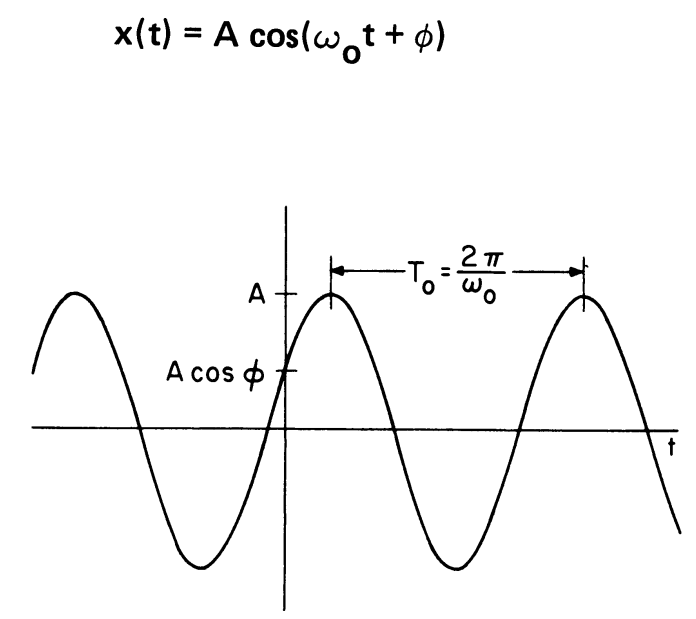
\includegraphics[height=0.8\textheight]{gambar/01.sinyal/01.slide_01}
	\end{figure}
\end{frame}

\begin{frame}{Sinyal sinusoidal waktu kontinu}
	\begin{figure}
		\centering
		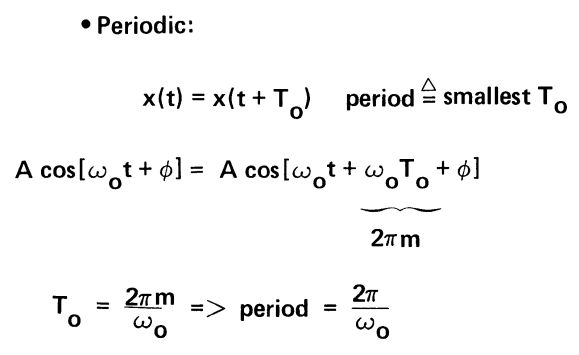
\includegraphics[height=0.7\textheight]{gambar/01.sinyal/01.slide_02_01}
	\end{figure}
\end{frame}

\begin{frame}{Sinyal sinusoidal waktu kontinu}
	\begin{figure}
		\centering
		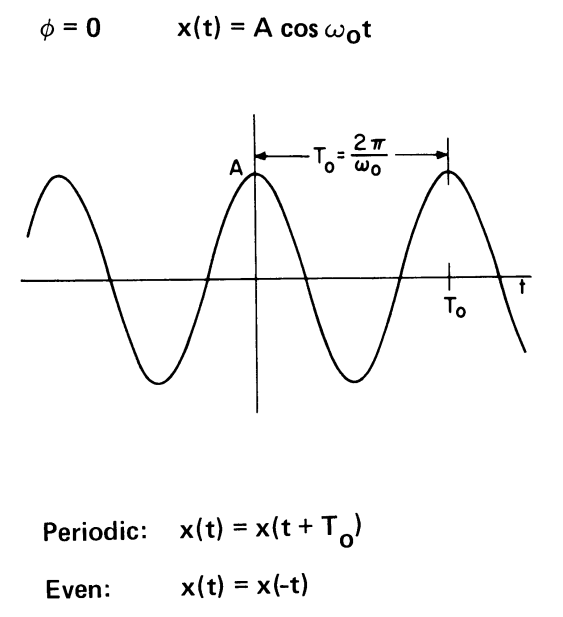
\includegraphics[height=0.8\textheight]{gambar/01.sinyal/01.slide_03}
	\end{figure}
\end{frame}

\begin{frame}{Sinyal sinusoidal waktu kontinu}
	\begin{figure}
		\centering
		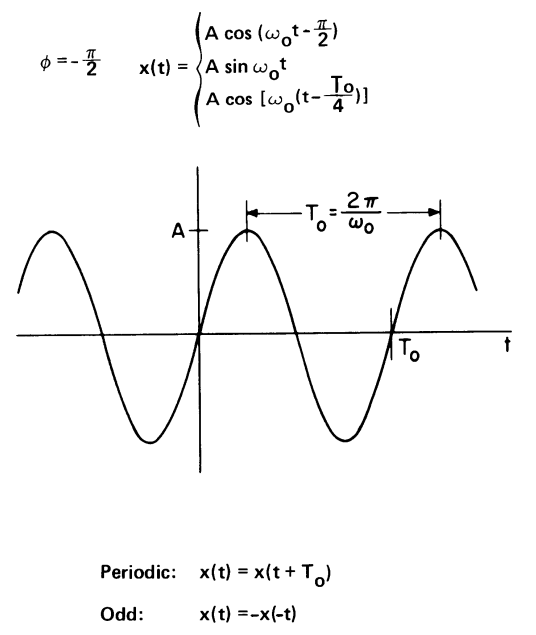
\includegraphics[height=0.8\textheight]{gambar/01.sinyal/01.slide_04}
	\end{figure}
\end{frame}

\section{Sinyal sinusoidal waktu diskret}
\begin{frame}{Sinyal sinusoidal waktu diskret}
	\begin{figure}
		\centering
		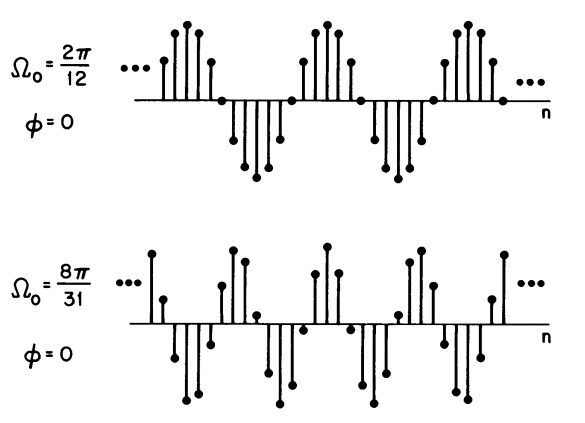
\includegraphics[height=0.8\textheight]{gambar/01.sinyal/01.slide_05}
	\end{figure}
\end{frame}

\begin{frame}{Sinyal sinusoidal waktu diskret}
	\begin{figure}
		\centering
		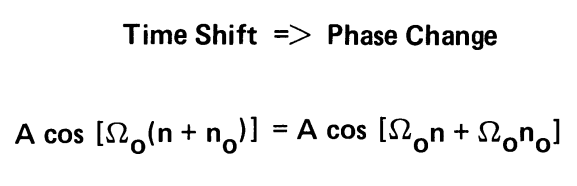
\includegraphics[height=0.3\textheight]{gambar/01.sinyal/01.slide_06}
	\end{figure}
\end{frame}

\begin{frame}{Sinyal sinusoidal waktu diskret}
	\begin{figure}
		\centering
		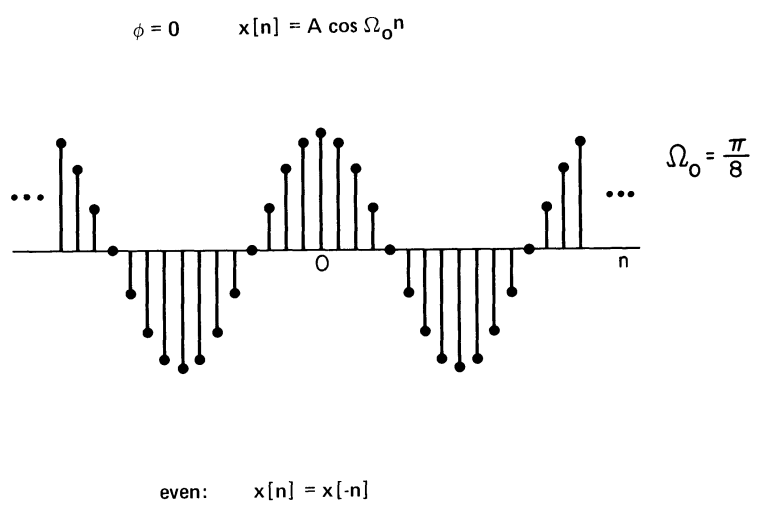
\includegraphics[height=0.8\textheight]{gambar/01.sinyal/01.slide_07}
	\end{figure}
\end{frame}

\begin{frame}{Sinyal sinusoidal waktu diskret}
	\begin{figure}
		\centering
		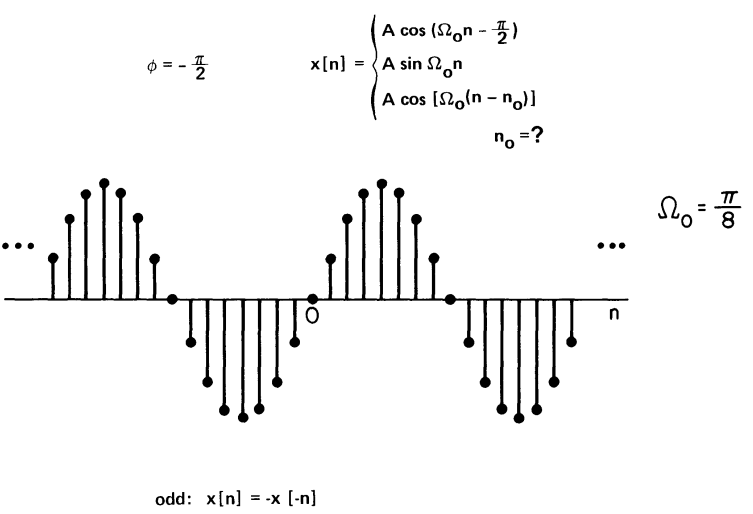
\includegraphics[height=0.8\textheight]{gambar/01.sinyal/01.slide_08}
	\end{figure}
\end{frame}

\begin{frame}{Sinyal sinusoidal waktu diskret}
	\begin{figure}
		\centering
		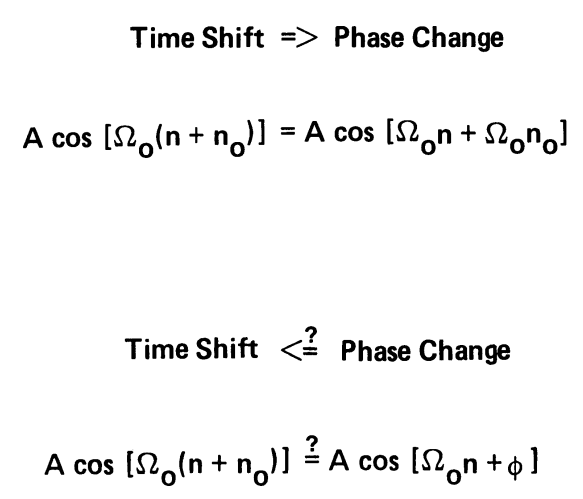
\includegraphics[height=0.8\textheight]{gambar/01.sinyal/01.slide_09}
	\end{figure}
\end{frame}

\begin{frame}{Sinyal sinusoidal waktu diskret}
	\begin{figure}
		\centering
		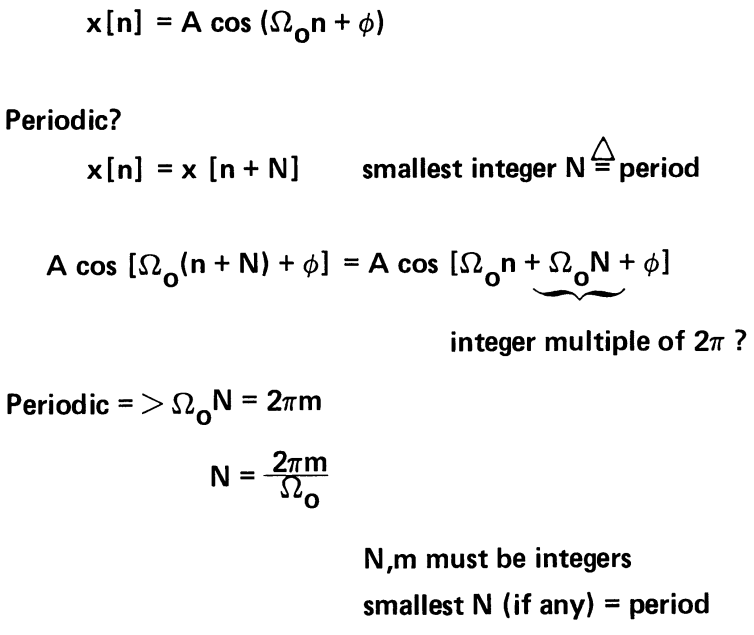
\includegraphics[height=0.8\textheight]{gambar/01.sinyal/01.slide_10}
	\end{figure}
\end{frame}

\begin{frame}{Sinyal sinusoidal waktu diskret}
	\begin{figure}
		\centering
		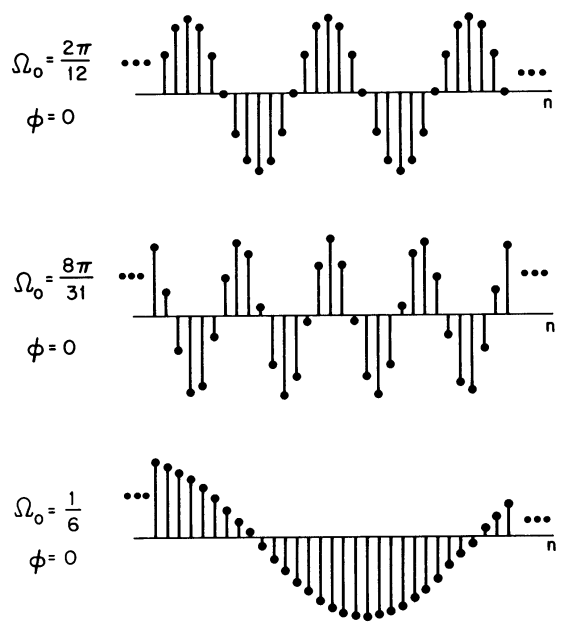
\includegraphics[height=0.8\textheight]{gambar/01.sinyal/01.slide_11}
	\end{figure}
\end{frame}

\begin{frame}{Sinyal sinusoidal waktu diskret}
	\begin{figure}
		\centering
		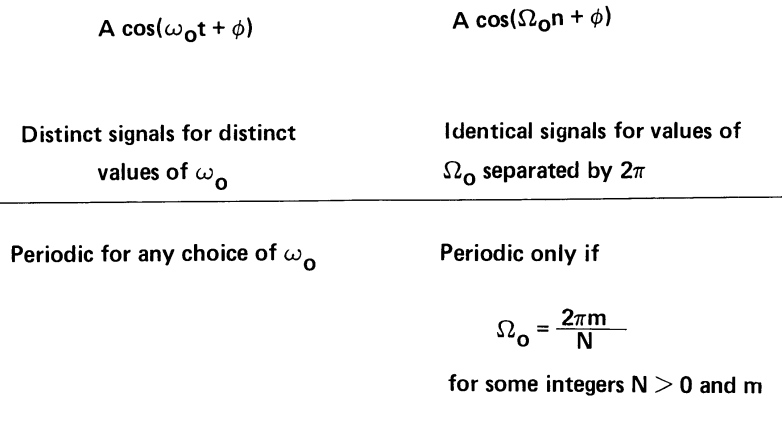
\includegraphics[height=0.8\textheight]{gambar/01.sinyal/01.slide_12}
	\end{figure}
\end{frame}

\section{Sinyal sinusoidal saat frekuensinya berbeda}
\begin{frame}{Sinyal sinusoidal saat frekuensinya berbeda}
	\begin{figure}
		\centering
		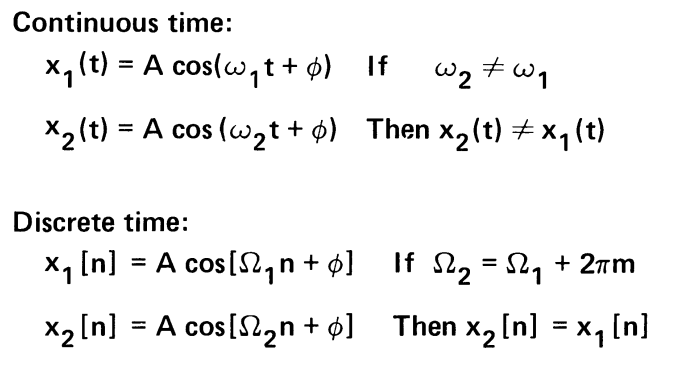
\includegraphics[height=0.8\textheight]{gambar/01.sinyal/01.slide_13}
	\end{figure}
\end{frame}

\section{Sinyal eksponensial riil waktu kontinu}
\begin{frame}{Sinyal eksponensial riil waktu kontinu}
	\begin{figure}
		\centering
		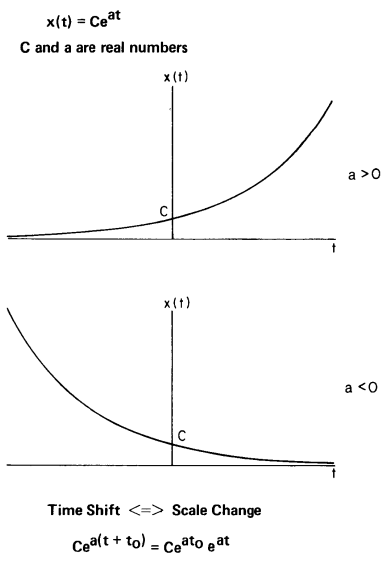
\includegraphics[height=0.8\textheight]{gambar/01.sinyal/01.slide_14}
	\end{figure}
\end{frame}

\section{Sinyal eksponensial riil waktu diskret}
\begin{frame}{Sinyal eksponensial riil waktu diskret}
	\begin{figure}
		\centering
		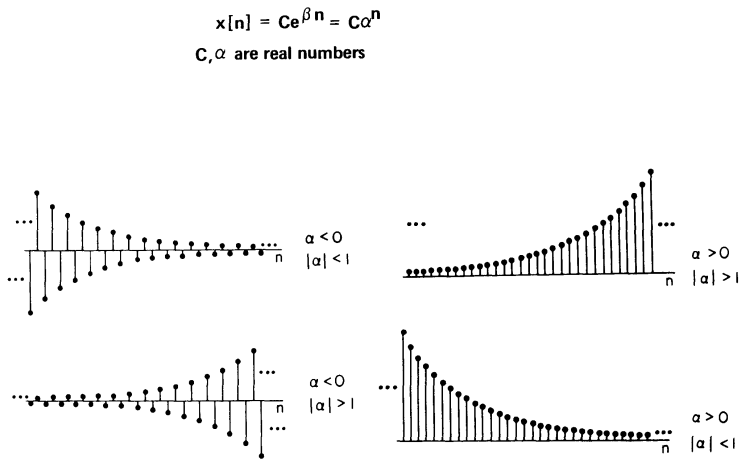
\includegraphics[height=0.8\textheight]{gambar/01.sinyal/01.slide_15}
	\end{figure}
\end{frame}

\section{Sinyal eksponensial kompleks waktu kontinu}
\begin{frame}{Sinyal eksponensial kompleks waktu kontinu}
	\begin{figure}
		\centering
		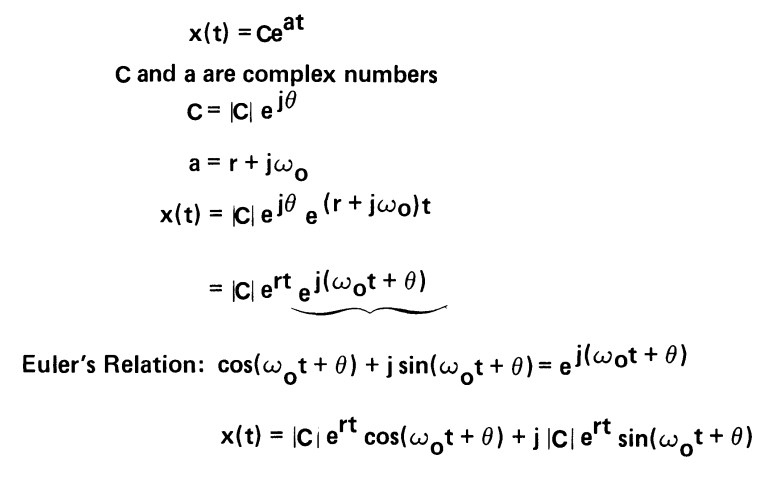
\includegraphics[height=0.8\textheight]{gambar/01.sinyal/01.slide_16}
	\end{figure}
\end{frame}

\begin{frame}{Sinyal eksponensial kompleks waktu kontinu}
	\begin{figure}
		\centering
		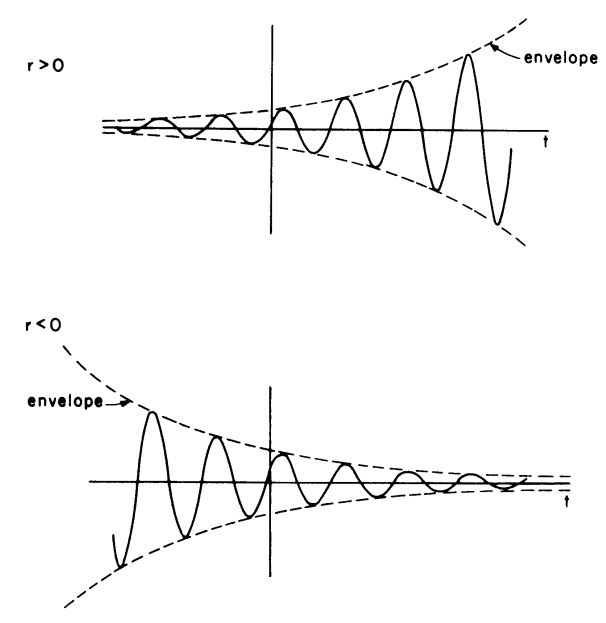
\includegraphics[height=0.8\textheight]{gambar/01.sinyal/01.slide_17}
	\end{figure}
\end{frame}

\section{Sinyal eksponensial kompleks waktu diskret}
\begin{frame}{Sinyal eksponensial kompleks waktu diskret}
	\begin{figure}
		\centering
		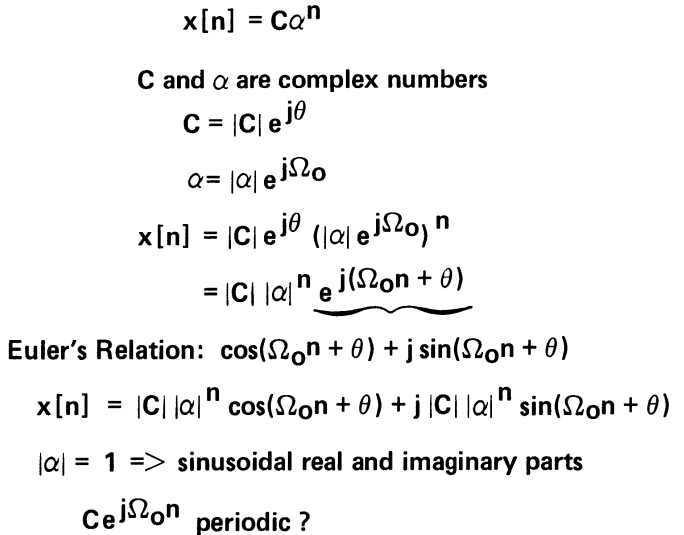
\includegraphics[height=0.8\textheight]{gambar/01.sinyal/01.slide_18}
	\end{figure}
\end{frame}

\begin{frame}{Sinyal eksponensial kompleks waktu diskret}
	\begin{figure}
		\centering
		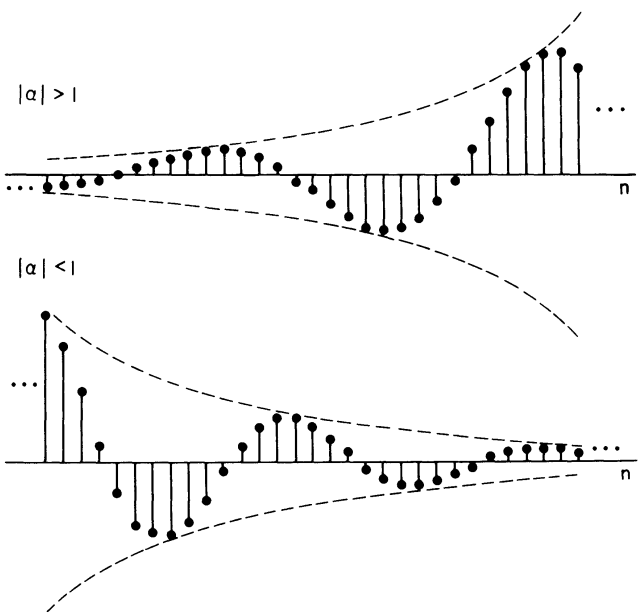
\includegraphics[height=0.8\textheight]{gambar/01.sinyal/01.slide_19}
	\end{figure}
\end{frame}

\section{Unit Step \& Unit Impulse}
\begin{frame}{Unit Step \& Unit Impulse}
	\begin{figure}
		\centering
		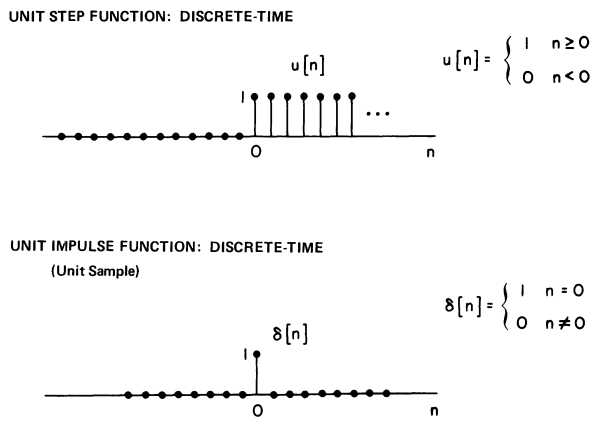
\includegraphics[height=0.8\textheight]{gambar/01.sinyal/02.slide_01}
	\end{figure}
\end{frame}

\begin{frame}{Unit Impulse Sequence}
	\begin{figure}
		\centering
		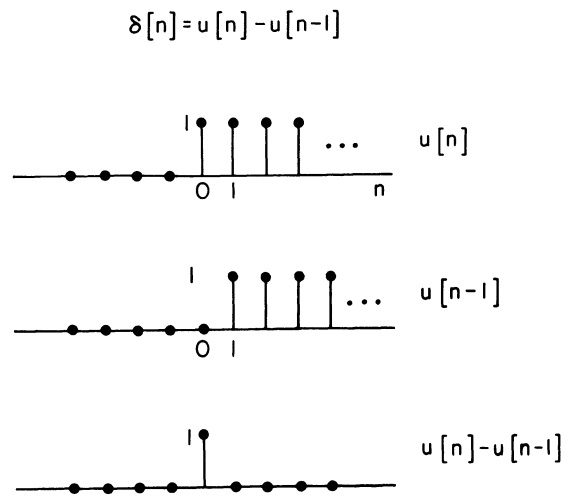
\includegraphics[height=0.8\textheight]{gambar/01.sinyal/02.slide_02}
	\end{figure}
\end{frame}

\begin{frame}{Unit Step Sequence}
	\begin{figure}
		\centering
		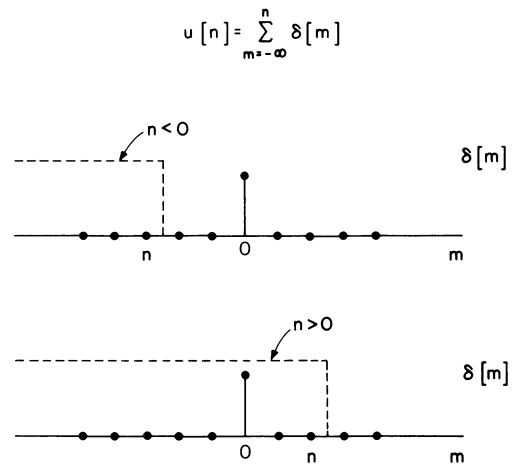
\includegraphics[height=0.8\textheight]{gambar/01.sinyal/02.slide_03}
	\end{figure}
\end{frame}

\begin{frame}{Unit Step Sequence}
	\begin{figure}
		\centering
		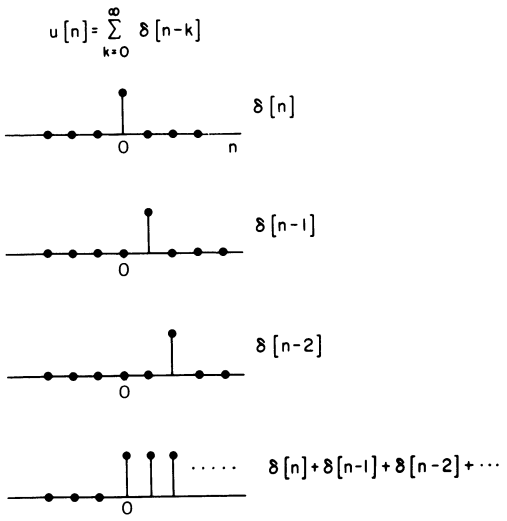
\includegraphics[height=0.8\textheight]{gambar/01.sinyal/02.slide_04}
	\end{figure}
\end{frame}

\begin{frame}{Unit Step Function Waktu Kontinu}
	\begin{figure}
		\centering
		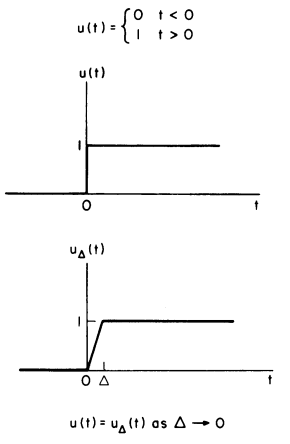
\includegraphics[height=0.8\textheight]{gambar/01.sinyal/02.slide_05}
	\end{figure}
\end{frame}

\begin{frame}{Unit Impulse Function}
	\begin{figure}
		\centering
		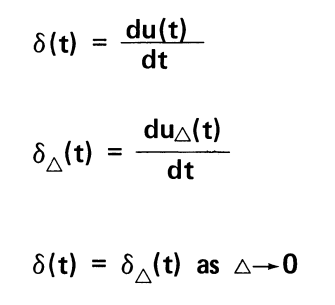
\includegraphics[height=0.4\textheight]{gambar/01.sinyal/02.slide_06}
	\end{figure}
\end{frame}

\begin{frame}{Unit Impulse Waktu Kontinu}
	\begin{figure}
		\centering
		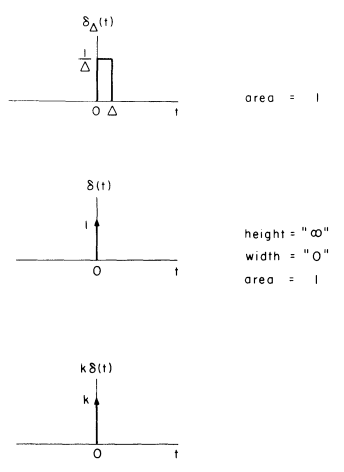
\includegraphics[height=0.8\textheight]{gambar/01.sinyal/02.slide_07}
	\end{figure}
\end{frame}

\begin{frame}{Unit Step Waktu Kontinu}
	\begin{figure}
		\centering
		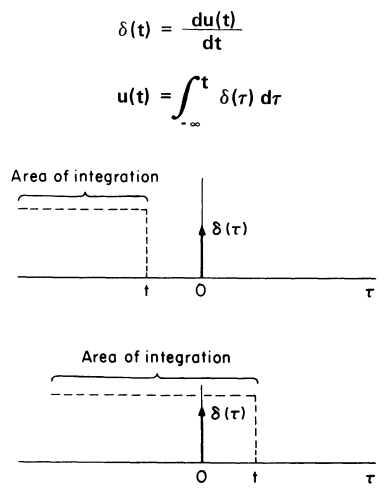
\includegraphics[height=0.8\textheight]{gambar/01.sinyal/02.slide_08}
	\end{figure}
\end{frame}

\end{document}

